% Drawing 161-6/02-6 -- folder 161-6, batch 02, archive page 25 (PDF page 26).
% Transcription: à gauche, un grand croquis : une grande courbe fermée contenant un disque (avec un trait intérieur, comme un rayon), un second domaine arrondi accolé au premier par-dessous et à droite, une boucle en pétale attachée à ce second domaine, une petite figure ramifiée (une tige double portant des branches en doigts) attachée au premier disque, et, à part, un court trait oblique.
% Kind: closed curve containing two adjoining discs, a loop and a branched figure. Method 2 (schematic redraw from the facsimile). Status: ok.
% Notes: Ink sketch. A large closed curve (through points read on his outline). Inside: a disc at the left (a circle), with an inner stroke like a radius; a second rounded domain adjoining it below and to the right, drawn as a curve that leaves the first disc at its upper right, makes a corner and returns to the foot of the first disc (both ends on the circle); a petal-shaped loop attached to the second domain at its upper right; a branched figure attached to the first disc at its upper right: a double stem (its left stroke heavy, its right stroke running on into the upper right lobe) and an outline with three fingers, a narrow one going up at the left and two rounded lobes at the right, one above the other, each finger with a short stroke inside; a short arc above the disc running into the stem; apart, at the upper right, a short oblique stroke, heavy at its upper end. The transcription's note says « deux disques accolés »: the second is not a full circle but a domain bounded in part by the first disc. Redrawn 2026-11-10 (issue 128). Question settled by a machine pass on the facsimile, 2026-11-12 (page): the second « disque » is not a full circle: its outline leaves the first disc and returns to it, so that it is bounded in part by the first disc; the drawing stands. 2026-11-13, Claude Opus 5.5, issue 147, overlay check: not compiled (no TeX in the session); the TikZ was rasterised by a local interpreter and laid over the 236 ppi scan rendered at 400 dpi. The large curve, the discs and the loop lie on their ink to within about one unit. Changed: the branched figure redrawn from a 17 pixels per unit crop: its outline through thirty points moved onto the ink (it has three fingers, not four), its stem and the three inner strokes fitted by least squares; each lies on its ink to within about half a unit. Not checked by a reader.
% Coordinates: 1 unit = 1 mm = 1/100 of the crop width (bbox in page fractions: [0.13, 0.34, 0.5, 0.6]).
% Redrawn by Claude (claude-fable-5-2), issue #128, 2026-11-10; not checked by a human; not compiled (no TeX in the session); overlay-checked on the scan by Claude Opus 5.5, issue #147, 2026-11-13, not compiled (no TeX in the session).
% Rights: reproduces part of the work -- behind RENDER_TRANSCRIPTS, never published by itself.
\documentclass[tikz,border=3pt]{standalone}
\usepackage{amsmath,amssymb}
\usetikzlibrary{patterns,arrows.meta}
\tikzset{pencil/.style={black!45}, struck/.style={black!35}, mpt/.style={circle,draw,inner sep=1.3pt}, pt/.style={circle,fill,inner sep=0.9pt}, opt/.style={circle,draw,fill=white,inner sep=1.1pt}}
\begin{document}
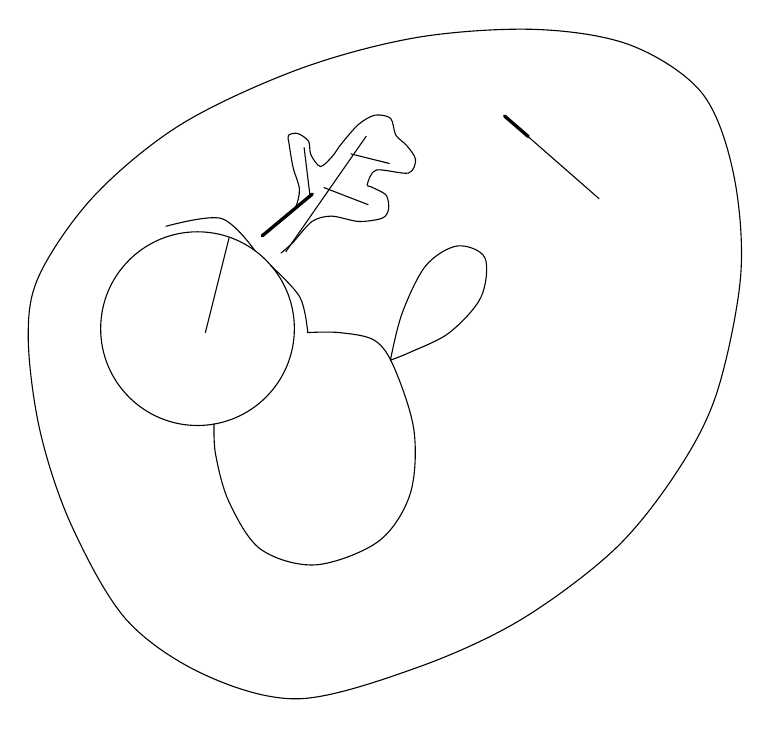
\begin{tikzpicture}[x=1mm,y=1mm,line cap=round,line join=round,font=\scriptsize]
\draw plot[smooth cycle, tension=0.55] coordinates {(70,-9) (82,-11) (91,-17) (95,-27) (96,-40) (93,-55) (88,-65) (80,-75) (68,-84) (55,-90) (40,-94) (28,-91) (18,-84) (11,-72) (7,-60) (5.5,-48) (7,-40) (14,-30) (25,-21) (40,-14) (55,-10)};
\draw (27,-47) circle[radius=12.3];
\draw (31,-35.5) -- (28,-47.5);
\draw plot[smooth, tension=0.55] coordinates {(36.3,-39) (40,-43) (41,-47.5)};
\draw plot[smooth, tension=0.55] coordinates {(41,-47.5) (45,-47.5) (49.5,-48.5) (52,-52) (54.5,-60) (54,-68) (50,-74) (42,-77) (35,-75) (31,-69) (29.3,-63) (29.1,-59.1)};
\draw plot[smooth, tension=0.55] coordinates {(51.5,-51) (53,-45) (56,-39) (60,-36.5) (63.5,-38) (63,-43) (59,-47.5) (54,-50) (51.5,-51)};
\draw plot[smooth, tension=0.55] coordinates {(23,-34) (30,-33) (34.3,-37.1)};
\draw plot[smooth, tension=0.5] coordinates {(35.74,-34.84) (37.74,-33.23) (39.4,-31.67) (39.94,-29.3) (39.14,-26.54) (38.62,-23.48) (38.55,-22.44) (39.74,-22.22) (41.1,-23.2) (41.39,-24.9) (42.61,-26.41) (44.14,-25.1) (45.22,-23.59) (47.45,-21.06) (49.53,-19.89) (51.52,-20.29) (52.18,-22.42) (53.56,-23.74) (54.69,-25.51) (53.79,-27.24) (49.68,-26.86) (48.55,-28.7) (48.98,-28.96) (50.95,-30.05) (51.26,-31.81) (50.48,-32.96) (47.5,-33.39) (44,-32.71) (41.53,-33.4) (39.08,-36.1) (37.6,-37.4)};
\draw[very thick] (35.22,-35.21) -- (41.58,-29.91);
\draw (38.22,-37.22) -- (48.42,-22.57);
\draw (40.54,-24.02) -- (41.28,-30.09);
\draw (46.49,-24.81) -- (51.36,-26.02);
\draw (43.07,-29.09) -- (48.66,-31.25);
\draw (66,-20) -- (78,-30.5);
\draw[very thick] (66,-20) -- (69,-22.6);
\end{tikzpicture}
\end{document}
